\documentclass[a4paper, oneside, 11pt, pointlessnumbers, headsepline]{scrbook}

% Get the necessary packages for the document.
% Set to english language and utf8.
\usepackage[english]{babel}
\usepackage[utf8]{inputenc}

% Some packages for symbols we need within the tutorial.
\usepackage{dingbat}
\usepackage{marvosym}

% For the sourcecode.
\usepackage{listings}

% For the links etc.
\usepackage[pdfborder={0 0 0}]{hyperref}

% For the pdf-graphics.
\usepackage{graphicx}

% The steamroller tactics to fix figures and so on.
\usepackage{float}

% This is for tables which are to long to be shown on one page.
\usepackage{longtable}

% This package is for the directory tree structures
\usepackage{dirtree}

% We need this package for some color within the document.
\usepackage{color}

% This is the package for the margin-nodes.
\usepackage[color=white, bordercolor=white]{todonotes}

\usepackage{amsfonts}
\usepackage{setspace}
\usepackage{ae,aecompl}

\usepackage[automark]{scrpage2}

\usepackage[margin=0.5cm,indention=-3em,font={sf},labelfont={bf,sf},format=hang]{caption}
% Get the new commands we defined for this document.
% The name of Kieker, just for the case that the design of this should change.
\newcommand{\Kieker}{\textsf{Kieker}}

% The current version-string.
\newcommand{\version}{1.5-trunk}

% The single parts of Kieker and some files.
\newcommand{\KiekerMonitoringPart}{\textsf{Kieker.Monitoring}}
\newcommand{\KiekerAnalysisPart}{\textsf{Kieker.Analysis}}
\newcommand{\analysisJar}{kieker-analysis-\version.jar}
\newcommand{\monitoringJar}{kieker-monitoring-\version.jar}
\newcommand{\commonJar}{kieker-common-\version.jar}
\newcommand{\toolsJar}{kieker-tools-\version.jar}
\newcommand{\commonsLoggingJar}{commons-logging-1.1.1.jar}
\newcommand{\monitoringPropertiesFile}{kieker.monitoring.properties}
\newcommand{\analysisPropertiesFile}{kieker.analysis.properties}
\newcommand{\logFourJPropertiesFile}{log4j.properties}
\newcommand{\aopFile}{aop.xml}

% The complete url where to find Kieker.
\newcommand{\KiekerURL}{\url{http://sourceforge.net/projects/kieker/files}}

% This is how we call the kieker directory.
\newcommand{\KiekerDir}{kieker-\version{}}%{$<$KIEKER-DIR$>$}

% These commands are necessary to mark classes, methods and files within the document.
\newcommand{\class}[1]{\texttt{#1}}
\newcommand{\method}[1]{\textit{#1}}
\newcommand{\dir}[1]{\texttt{#1}}
\newcommand{\file}[1]{\texttt{#1}}

% TODO command for our document
\newcommand{\TODO}[1]{\todo[inline,color=green!40]{TODO: #1}}

% These commands are for notifying the reader about something important.
\newcommand{\marginbox}[1]{\todo[noline]{#1}}
\newcommand{\notify}{\marginbox{\huge{\rightpointleft}}}
\newcommand{\warning}{\marginbox{\huge{\Stopsign}}}


% The following commands set the listings for the different (programming) languages correctly.
% For the first they use all nearly the same settings.
\newcommand{\setListing}[4]{
\lstset{
language=#1,          
numbers=#2,
basicstyle=#3,       	% the size of the fonts that are used for the code
showspaces=false,               % show spaces adding particular underscores
showstringspaces=false,         % underline spaces within strings
showtabs=false,                 % show tabs within strings adding particular underscores
%frame=shadowbox,	                % adds a frame around the code
frame=lrtb,
rulesepcolor=\color{black},
tabsize=2,	                % sets default tabsize to 2 spaces
captionpos=t,                   % sets the caption-position to bottom
breaklines=true,                % sets automatic line breaking
breakatwhitespace=false,        % sets if automatic breaks should only happen at whitespace
title=\lstname,                 % show the filename of files included with \lstinputlisting; also try caption instead of title
escapechar={#4}
}
}
\newcommand{\setJavaCodeListing}{\setListing{Java}{left}{\sffamily\scriptsize}{}}
\newcommand{\setBashListing}{\setListing{Bash}{none}{\sffamily\scriptsize}{°}}
\newcommand{\setXMLListing}{\setListing{XML}{none}{\sffamily\scriptsize}{}}


\pagestyle{scrheadings}
\clearscrheadfoot

\ifoot[\hrule\sffamily Kieker Developer Guide]{\hrule\sffamily Kieker Developer Guide} % \version{}
\ofoot[\hrule\sffamily\pagemark]{\hrule\sffamily\pagemark} 

% Set the title and everything.
\titlehead{
	\begin{center}
		
\includegraphics[height=25mm]{./figures/kieker-logo}\\
\href{http://kieker.sourceforge.net}{\sffamily\Large http://kieker.sourceforge.net}
	\end{center}
}

\title{%
\Huge\Kieker{} Developer Guide%\\[0.5ex] \Large{Continuous Monitoring and Analysis of Java Software Behavior}%
}
% \subtitle{---User Guide---}
\author{\sffamily Kieker Project}
\date{\sffamily\today}
\publishers{\normalsize\sffamily
%\flushleft

\includegraphics[height=2.5cm]{./figures/caulogo}\\[0.5ex]
Software Engineering Group\\ University of Kiel, Germany
}

% Here we go.
\begin{document}
  % We want a table of contents seperated from the rest of the text.
  \maketitle
  \tableofcontents

  % Insert the other parts of the document.
\chapter{Introduction}
\input{sec-introduction.inc}

\chapter{Project Management}
\section{Subversion Repository}

We provide anonymous (read-only) access to the Kieker subversion repository:

\begin{compactitem}
\item \textbf{URL:}\\ \url{https://samoa.informatik.uni-kiel.de/svn/projects/kieker/software/kieker/}
\item \textbf{Username:} anonymous
\item \textbf{Password:} anonymous
\end{compactitem}

\medskip

\noindent In order to request write access, please send an e-mail to \texttt{avh@informatik.uni-kiel.de}.

\section{Mailing Lists}

You should register to the following to mailing lists:

\begin{itemize}
\item \textbf{kieker-users@sourceforge.net:}\\ \url{https://lists.sourceforge.net/lists/listinfo/kieker-users}
\item \textbf{kieker-developers@sourceforge.net:}\\ \url{https://lists.sourceforge.net/lists/listinfo/kieker-developers}
\end{itemize}


\section{Bug Tracker}

The bug tracker can be accessed via: 

\begin{itemize}
\item[] \url{http://sourceforge.net/tracker/?group_id=212691&atid=1022738}
\end{itemize}




\chapter{Build and Development Environment}
\section{Ant Build}

Ant is used as the build tool for Kieker. %
The important ant targets included in the \texttt{build.xml} file are:

\begin{itemize}
\item \textbf{build-all:} This is the default target that compiles the Kieker %
artifacts and creates the following jar/war files in the \texttt{dist/} directory:
\begin{compactitem}
\item \texttt{kieker-analysis-1.5-trunk.jar} 
\item \texttt{kieker-common-1.5-trunk.jar}
\item \texttt{kieker-monitoring-1.5-trunk.jar}
\item \texttt{kieker-monitoring-servlet-1.5-trunk.war}
\item \texttt{kieker-tools-1.5-trunk.jar}
\end{compactitem}
\item \textbf{javadoc:} Executes Javadoc to create the API documentation in HTML. %
After a successful execution, open \texttt{build/javadoc/index.html} in your %
Web browser.
\item \textbf{run-tests-junit:} Runs the JUnit tests and creates a HTML report %
of the results. 
\item \textbf{run-test$[$s$]$-*:} Additional regression tests mostly employing %
AspectJ for instrumentation. 
\item \textbf{release:} Creates the following Kieker release files in the %
\texttt{dist/release/} directory:
\begin{compactitem}
\item \texttt{kieker-<version>\_javadoc.(zip|tar.gz)}
\item \texttt{kieker-<version>\_binaries.(zip|tar.gz)}
\item \texttt{kieker-<version>\_sources.(zip|tar.gz)}
\item \texttt{kieker-<version>\_examples-JPetStoreExample.(zip|tar.gz)}
\item \texttt{kieker-<version>\_examples-MySimpleKiekerAspectJExample.(zip|tar.gz)}
\item \texttt{kieker-<version>\_examples-MySimpleKiekerJMSExample.(zip|tar.gz)}
\item \texttt{kieker-<version>\_examples-OverheadEvaluationMicrobenchmark.(zip|tar.gz)}
\end{compactitem}
\end{itemize}

\section{IDE-Specific Project Configuration}

This section describes how to create a project for developing with the 
Kieker sources in different IDEs.

\subsection{Netbeans}

You create a Netbeans project for the Kieker trunk as follows:

\begin{compactenum}
\item File->New Project\ldots and select \textit{Java Free-Form Project} and 
follow the wizard and answer the dialogs as follows:

\begin{compactenum}
\item \textbf{Name and Location (Fig.~\ref{fig:nb:location}):} %

Select Kieker's \texttt{trunk/} directory as the project location and th wizard will %
complete the missing information based on the existing \texttt{build.xml} file.

\begin{figure}[H]\centering
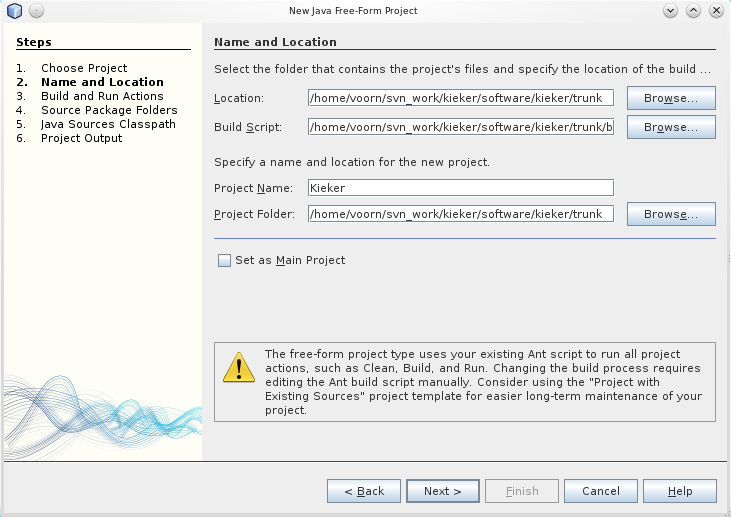
\includegraphics[scale=0.4]{figures/netbeans-NameAndLocation}
\caption{}
\label{fig:nb:location}
\end{figure}

\item \textbf{Build and Run Actions (Fig.~\ref{fig:nb:buildRun}):} %

Complete the information as shown in Fig.~\ref{fig:nb:buildRun}.

\begin{figure}[H]\centering
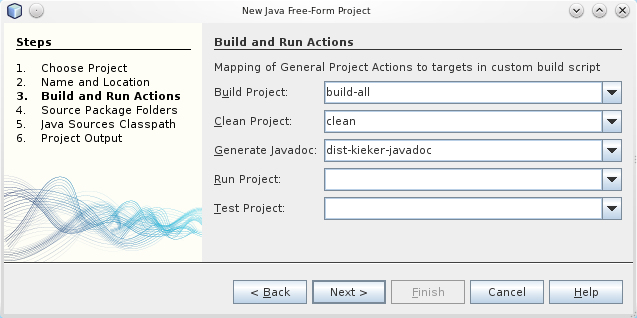
\includegraphics[scale=0.4]{figures/netbeans-BuildAndRun}
\caption{}
\label{fig:nb:buildRun}
\end{figure}

\item \textbf{Source Package Folders (Fig.~\ref{fig:nb:sourcePackageFolders}):} %

\textbf{Add} alls subdirectories of \texttt{src/} and all subdirectories of %
\texttt{ test/} (except for \texttt{test/META-INF/}) to the list of %
\textit{Source Package Folders}. %
\textbf{Remove all \textit{Test Package Folders} entries.}

\begin{figure}[H]\centering
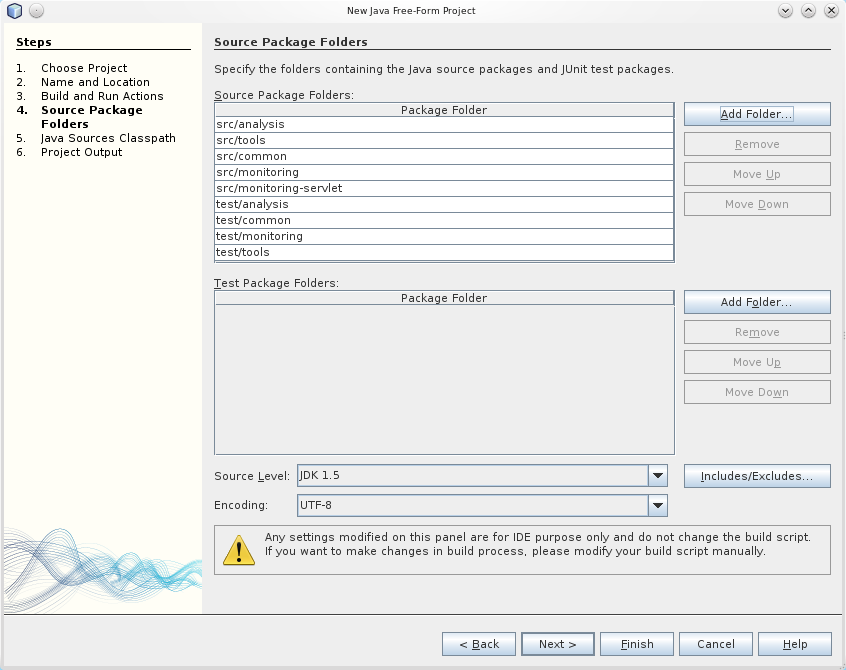
\includegraphics[scale=0.4]{figures/netbeans-SourcePackageFolders}
\caption{}
\label{fig:nb:sourcePackageFolders}
\end{figure}

\item \textbf{Java Sources Classpath (Fig.~\ref{fig:nb:sourcesclasspath}):} %

\textbf{\underline{Un}check} the option \textit{Separate Classpath for Each Source Package Folder} and %
\textbf{add} all .jar files included in the \texttt{lib/} directory.

\begin{figure}[H]\centering
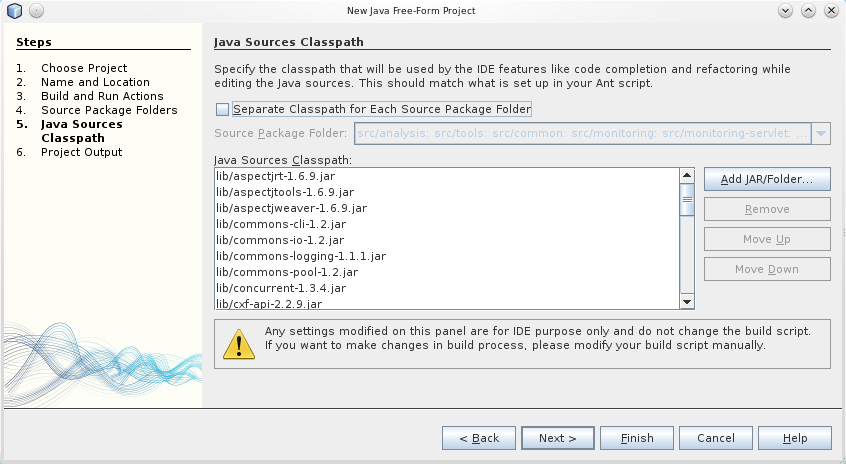
\includegraphics[scale=0.4]{figures/netbeans-SourcesClasspath}
\caption{}
\label{fig:nb:sourcesclasspath}
\end{figure}

\item \textbf{Project Output (Fig.~\ref{fig:nb:projectOutput})} %

Simply skip this dialog without any changes and finish the wizard by clicking %
on the \textbf{Finish} button.

\begin{figure}[H]\centering
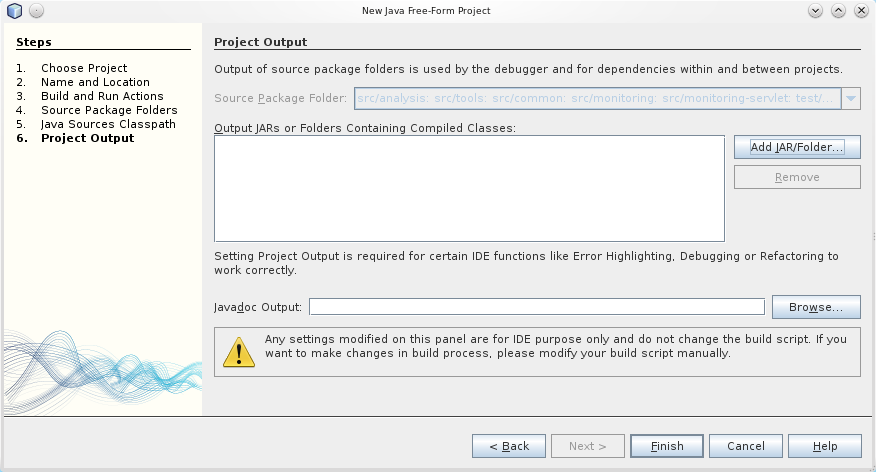
\includegraphics[scale=0.4]{figures/netbeans-ProjectOutput}
\caption{}
\label{fig:nb:projectOutput}
\end{figure}

\item Kieker should now appear in the list of projects, as shown in Fig.~\ref{fig:nb:projectTree}.  

\begin{figure}[H]\centering
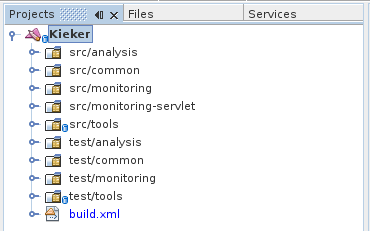
\includegraphics[scale=0.4]{figures/netbeans-ProjectTree}
\caption{}
\label{fig:nb:projectTree}
\end{figure}
\end{compactenum}
\end{compactenum}

\subsection{Eclipse}

You create an Eclipse project for the Kieker trunk as follows:

\begin{compactenum}
\item Kieker includes two sample files to create an Kieker Eclipse project: %
\begin{compactitem}
\item \texttt{eclipse-classpath.sample}
\item \texttt{eclipse-project.sample} 
\end{compactitem}

\noindent \textbf{Copy} these files to \texttt{.classpath} and \texttt{.project} respectively.

\item Open the Java project creation wizard by selecting File->New->Java Project.
\begin{compactenum}
\item \textbf{Create a Java Project (Fig.~\ref{fig:eclipse:newProject}):} %

\textbf{\underline{Un}check} \textit{Use default location} and select Kieker's %
\texttt{trunk/} directory from your filesystem. Rename the project to ``Kieker''. 

\begin{figure}[H]\centering
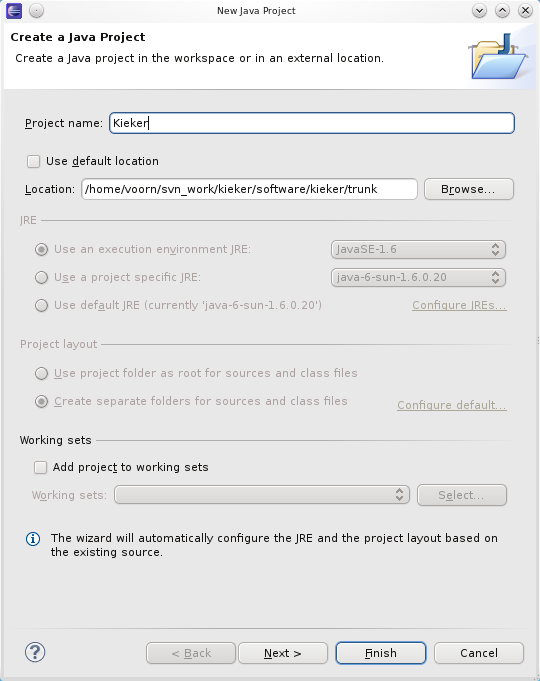
\includegraphics[scale=0.4]{figures/eclipse-NewProject}
\caption{}
\label{fig:eclipse:newProject}
\end{figure}

\item \textbf{Java Settings (Fig.~\ref{fig:eclipse:javaSettings}):} %

All settings in this dialog should be imported correctly from the \texttt{.project} %
and \texttt{.classpath} files. Simply skip this dialog without any changes and finish the wizard by clicking %
on the \textbf{Finish} button.

\begin{figure}[H]\centering
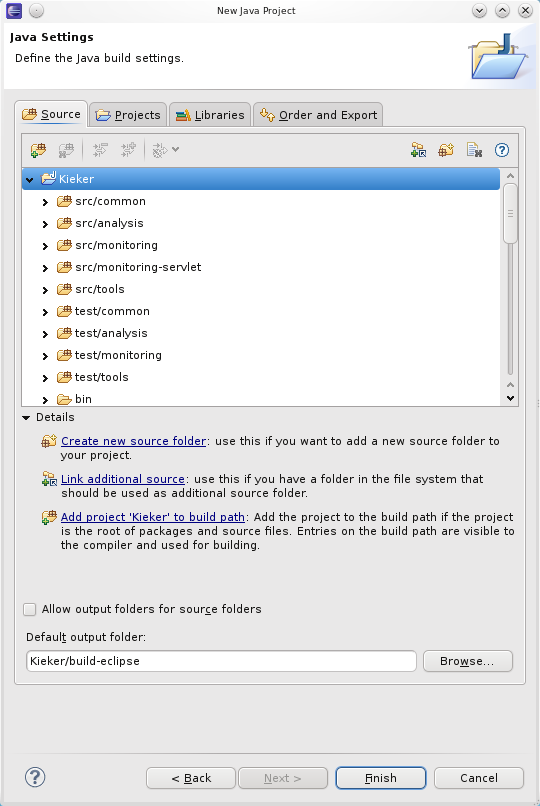
\includegraphics[scale=0.4]{figures/eclipse-JavaSettings}
\caption{}
\label{fig:eclipse:javaSettings}
\end{figure}

\item Kieker should now appear in the list of projects, as shown in Fig.~\ref{fig:eclipse:projectTree}.  

\begin{figure}[H]\centering
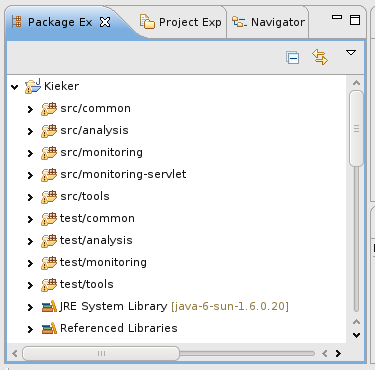
\includegraphics[scale=0.4]{figures/eclipse-ProjectTree}
\caption{}
\label{fig:eclipse:projectTree}
\end{figure}

\end{compactenum}
\end{compactenum}

\section{Continuous Integration}

Not yet performned, but we might evaluate the following tools

\begin{compactitem}
\item CruiseControl: \url{http://cruisecontrol.sourceforge.net/}
\item Hudson: \url{http://hudson-ci.org/}
\end{compactitem}




\chapter{Creating a Release}
\textbf{Checklist for creating a release version}

\begin{compactenum}
\item Tag the \dir{trunk/} to work on a frozen copy:
\setBashListing
\begin{lstlisting}
 svn cp trunk/  tags/<version>/
\end{lstlisting}
\item Set the final release version number in the \file{build.xml}
\item Modify the \file{HISTORY} file
\item Commit the tag
\item Export a clean version of the tag from the svn:
\setBashListing
\begin{lstlisting}
svn export \
 http://samoa.informatik.uni-kiel.de/[...]/tags/1.2 kieker-1.2-export \
 --username=USER --password=PASS
\end{lstlisting}
\item \textbf{Build the release files}
\setBashListing
\begin{lstlisting}
ant release
\end{lstlisting}
\item \textbf{Test the source release:} \textit{--- Extract source release archive to a tmp directory}
\begin{compactenum}
\item Manually inspect contents
\item Test build:
\setBashListing
\begin{lstlisting}
ant
\end{lstlisting}
\item Execute JUnit tests
\setBashListing
\begin{lstlisting}
ant run-tests-junit
\end{lstlisting}
\item Execute integration tests (each test eventually terminates; some take quite a while)
\setBashListing
\begin{lstlisting}
ant run-tests-compileTimeWeaving-bookstore
ant run-tests-compileTimeWeaving-bookstore-synchronized
ant run-tests-compileTimeWeaving-bookstoreDB
ant run-tests-compileTimeWeaving-twoConcurrentMethodsExample
ant run-tests-loadTimeWeaving-bookstoreDifferentRecordTypes
ant run-tests-loadTimeWeaving-bookstoreFullInstrumentation
ant run-tests-loadTimeWeaving-executionOrderTest
ant run-test-storage
\end{lstlisting}
\end{compactenum}

\item \textbf{Test the binary release:} \textit{--- Extract binary release archive to a tmp directory}
\begin{compactenum}
\item Test wrapper scripts: \textbf{\textit{--- Linux \& Windows}}
\begin{compactitem}
\item \file{bin/convertLoggingTimestamp.sh} \textit{--- inspect generated \file{.html}/\file{.txt} files}
\setBashListing
\begin{lstlisting}
bin/convertLoggingTimestamp.sh \
 --timestamps 1283156545581511026 1283156546127117246
\end{lstlisting}
\item \file{bin/trace-analysis.sh}
\setBashListing
\begin{lstlisting}
bin/trace-analysis.sh --inputdirs examples/userguide/ch5--trace-monitoring-aspectj/testdata/tpmon-20100830-082225522-UTC/ --outputdir . --plot-Deployment-Component-Dependency-Graph --plot-Assembly-Component-Dependency-Graph --plot-Container-Dependency-Graph --plot-Deployment-Operation-Dependency-Graph --plot-Assembly-Operation-Dependency-Graph --plot-Aggregated-Deployment-Call-Tree --plot-Aggregated-Assembly-Call-Tree --print-Deployment-Equivalence-Classes --print-Assembly-Equivalence-Classes --plot-Aggregated-Deployment-Call-Tree --plot-Aggregated-Assembly-Call-Tree --short-labels

bin/trace-analysis.sh --inputdirs examples/userguide/ch5--trace-monitoring-aspectj/testdata/tpmon-20100830-082225522-UTC/ --outputdir . --select-traces  6488138950668976141 6488138950668976129 6488138950668976130 6488138950668976131 --plot-Deployment-Sequence-Diagrams --plot-Assembly-Sequence-Diagrams --plot-Call-Trees --print-Message-Traces --print-Execution-Traces  --short-labels
\end{lstlisting}

% \begin{lstlisting}
% bin/trace-analysis.sh \
%   -i examples/userguide/ch5--trace-monitoring-aspectj/testdata/tpmon-20100830-082225522-UTC/\
%   -o . --plot-Deployment-Operation-Dependency-Graph --plot-Assembly-Operation-Dependency-Graph
% 
% bin/trace-analysis.sh \
%   -i examples/userguide/ch5--trace-monitoring-aspectj/testdata/tpmon-20100830-082225522-UTC/\
%   -o . --plot-Deployment-Sequence-Diagrams --plot-Assembly-Sequence-Diagrams
%   --select-traces 6488138950668976192 6488138950668976197
% \end{lstlisting}
\item \file{bin/dotPic-fileConverter.sh}
\setBashListing
\begin{lstlisting}
bin/dotPic-fileConverter.sh . pdf ps png
\end{lstlisting}
\item \file{bin/logReplay.sh}
\setBashListing
\begin{lstlisting}
bin/logReplay.sh \
 -i examples/userguide/ch5--trace-monitoring-aspectj/testdata/tpmon-20100830-082225522-UTC/ \
 -k true -r false

diff -r examples/userguide/ch5--trace-monitoring-aspectj/testdata/tpmon-20100830-082225522-UTC/tpmon-20100830-082225582-UTC-Thread-2.dat \
 <replayed dat file>
\end{lstlisting}
\item \file{bin/mappingGenerator.sh} ---
\textit{Not really used so far}
\end{compactitem}

\item Execute user guide examples:

\begin{compactitem}
\item \dir{ch2--bookstore-application}
\setBashListing
\begin{lstlisting}
ant run-jar
\end{lstlisting}
\item \dir{ch2--manual-instrumentation} -- copy jars first
\setBashListing
\begin{lstlisting}
ant run-monitoring
ant run-analysis -Danalysis.directory=<DIR>
\end{lstlisting}
\item \dir{ch3-4--custom-components} -- copy jars first
\setBashListing
\begin{lstlisting}
ant run
\end{lstlisting}
\item \dir{ch5--trace-monitoring-aspectj} -- copy jars first
\setBashListing
\begin{lstlisting}
ant run
\end{lstlisting}
\item \dir{appendix-JMS} -- see instructions in user guide% appendix
\item \dir{JavaEEServletContainerExample} -- see instructions in user guide% appendix
\end{compactitem}
\item Check user guide PDF \file{doc/kieker-userguide.pdf}
\end{compactenum}

\item Copy \dir{dist/} to SVN tag and add to repository
\item Merge the \dir{tag/}'s changes (if such) back to the \dir{trunk/}
\item \textbf{Publish release files}\\
{\scriptsize\url{https://sourceforge.net/apps/trac/sourceforge/wiki/Release files for download#Createoreditarelease}}\\
Uploads via \textit{Project Admin} $\rightarrow$ \textit{File Manager}
\begin{compactenum}
\item \dir{/}
\begin{compactenum}
\item \file{kieker-<version>\_binaries.zip|tar.gz}
\item \file{kieker-<version>\_sources.zip|tar.gz}
\item \file{kieker-userguide.pdf} (e.g., extracted from zip)
\end{compactenum}
\item \dir{/examples/}
\begin{compactenum}
\item \file{kieker-examples-JavaEEServletContainerExample.zip|tar.gz}
\end{compactenum}
\item \dir{/javadoc/}
\begin{compactenum}
\item \file{kieker-<version>\_javadoc.zip|tar.gz}
\end{compactenum}
\end{compactenum}
\item Upload HTML version of Javadoc API\\
Only via scp: {\scriptsize\texttt{SFUSER,kieker@web.sourceforge.net:/home/groups/k/ki/kieker/htdocs/}}\\
(An ftp client supporting scp can be used, of course)
\begin{compactenum}
\item Create directory \dir{<version>/doc/api/}
\item Upload contents of unzipped javadoc
\end{compactenum}
\end{compactenum}

\chapter{Testing}
\section{JUnit Tests}

\section{Integration Tests}

\chapter{Documentation}
\section{Javadoc API}

\section{User Guide}

\section{Developer Guide}

\section{Web Site}

\chapter{Architectural Details}
\section{Goals}

\begin{compactitem}
\item Low Overhead
\item Robustness 
\item Desgined for continuous operation
\end{compactitem}


\section{Design Decisions}

\chapter{Roadmap}
\input{sec-roadmap.inc}

\end{document}
 
